\section{The instrument in the wild}
\label{sec:wild}

\subsection{Two labellers, recovered exactly}
\label{sec:recovery}

\paragraph{Sea ice.} The labeller of~\cite{iqrah2023polar}, scaled with cloud and
shadow removal in~\cite{iqrah2024parallel}, applies HSV thresholds to each RGB patch
after background subtraction. The thresholds admit hue 0 to 185 while OpenCV hue
ranges 0 to 179, so hue and saturation constrain nothing and only the value channel
acts. A two-parameter grid search recovers the water constant in 17 of 17 folds.
Otsu and two min-max normalisations are recomputed on each $128 \times 128$ patch,
so a pixel's label depends on the framing of its crop. Regenerating once per scene
makes the labels exactly crop-invariant: crop unanimity is $1.0000$ on all 17 folds
for the repaired scheme against $0.9678$ for the original.

\paragraph{Floods.} Sen1Floods11 ships an expert label and an Otsu label for the
same 446 chips, and unlike the sea-ice case it publishes the constant, so the
recovery can be checked from outside. Recovery from the raw band gives 94.9\% pixel
agreement but sits 1.19\,dB low on all ten events with a published value. A bias of
one sign everywhere is a signature, not noise. Sweeping the smoothing radius,
the bias crosses zero at a $9 \times 9$ focal mean, where 10 of 10 events land within
0.25\,dB at 99.05\% agreement (\cref{fig:recovery}). The constant moves 5.57\,dB
across events, so no global threshold can express it and a model seeing the whole
chip can infer which event it is in and adapt.

\begin{figure}[tb]
\centering
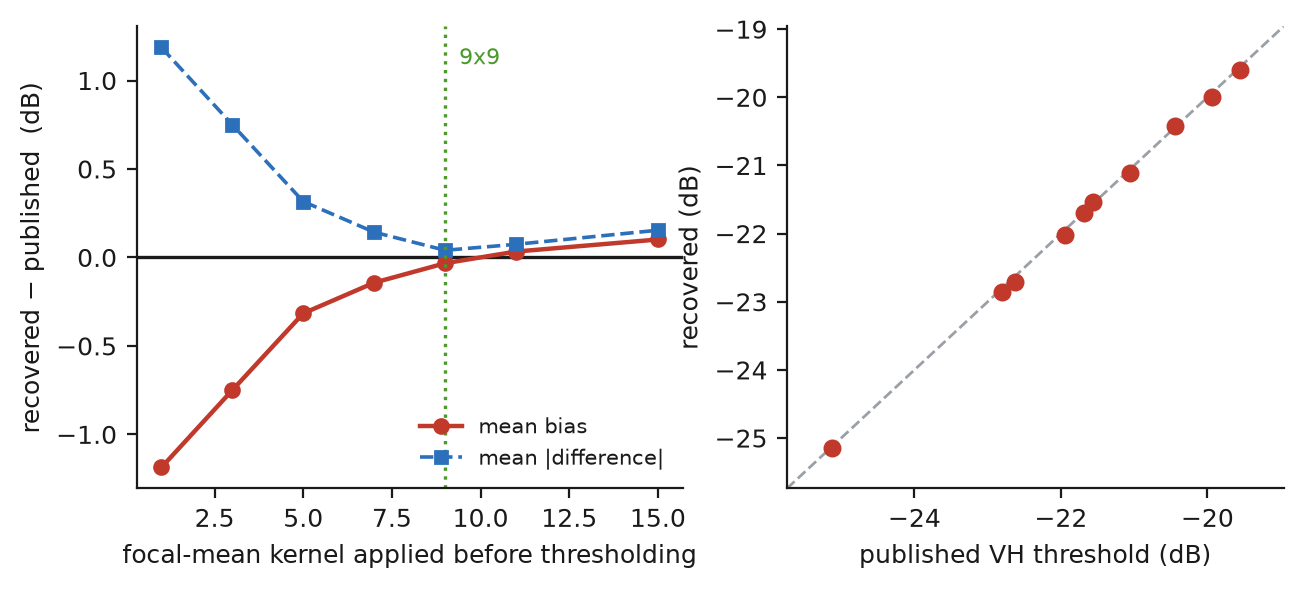
\includegraphics[width=\linewidth]{figures/label_generator_recovery.png}
\caption{Recovering the flood labeller. Left: bias and mean absolute difference
against the published thresholds as the smoothing kernel is swept. Right: recovered
against published threshold, one point per event.}
\label{fig:recovery}
\end{figure}

\subsection{Crop alignment on the sea-ice benchmark}

Sea-ice crops overlap about 33 times, so a source pixel is seen inside many crops,
and under the per-crop scheme those crops can disagree. For the 16 folds with
committed machine-readable results, $\A$ averages 13.58\% of covered pixels. The
model trained on crop-noisy labels reads $\kap=+0.1230$ (sd $0.0361$); the matched
control, trained on repaired labels and evaluated on identical pixels, reads
$+0.0157$. Their paired difference is $\mathbf{+0.1073}$ (sd $0.0333$,
$t=12.88$, positive in 16 of 16 folds, two-sided sign test $p=0.000031$).
\Cref{fig:wild} shows all machine-readable folds. The power formula returns a value
below two, where a paired variance cannot be estimated, so we do not quote a
required sample size.

The released text summary contains a rounded seventeenth row, but the corresponding
per-fold JSON is absent. Including it would change the paired difference to
$+0.1106$. We exclude that row from every headline result rather than silently
mixing machine-readable evidence with an unreconstructable summary.

\begin{figure}[tb]
\centering
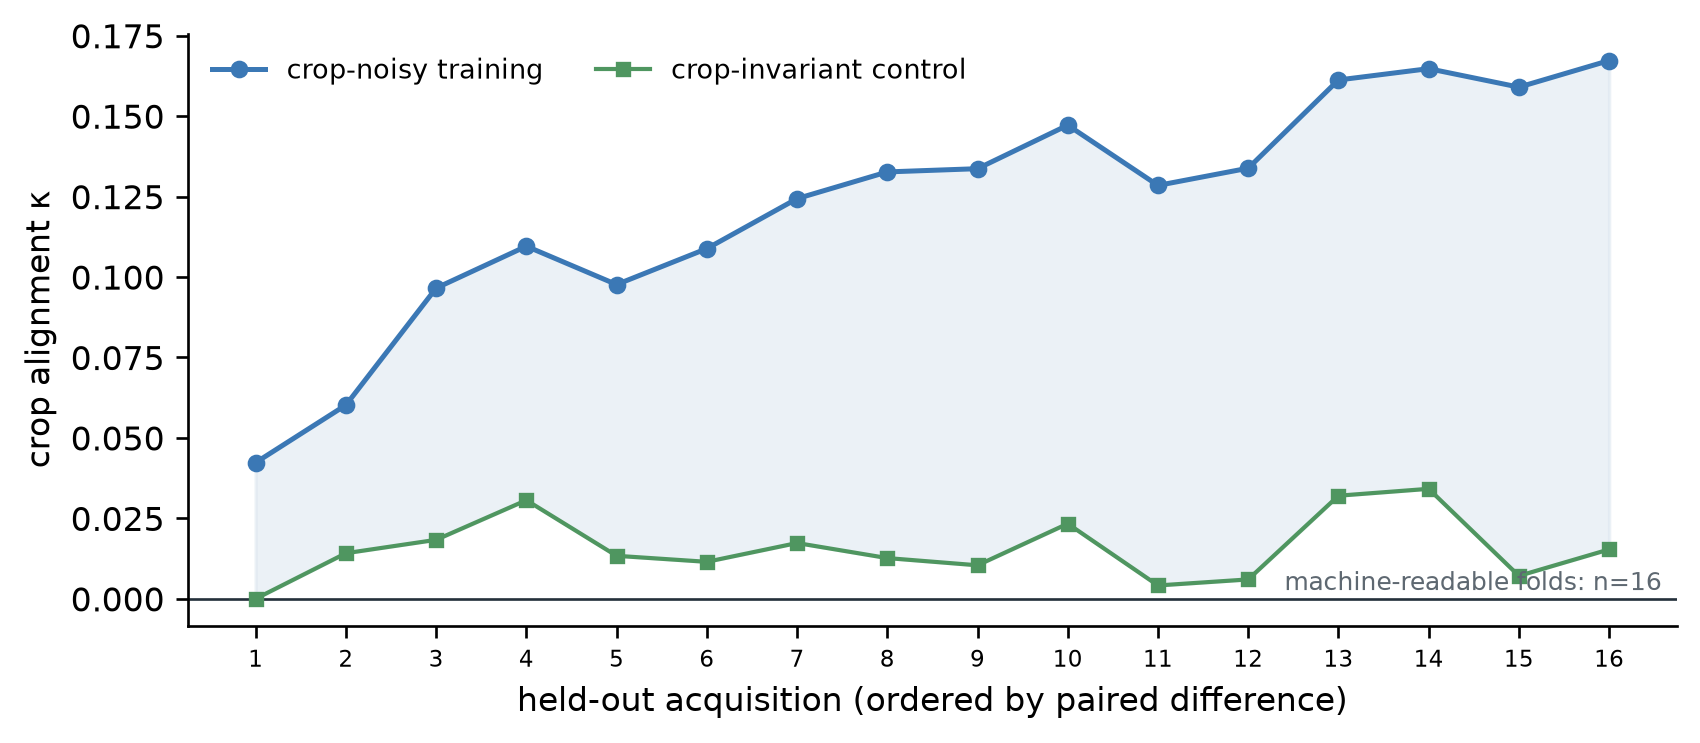
\includegraphics[width=\linewidth]{figures/crop_alignment_results.png}
\caption{Crop alignment for the 16 held-out acquisitions with machine-readable
evidence, each against its matched control. The zero line is the structural null of
\cref{prop:null}, not an estimated baseline.}
\label{fig:wild}
\end{figure}

We do not divide this by the calibrated contrast of \Cref{sec:calib} to express it
as a fraction of a fully closed-loop labeller. The two were measured on different
crop grids, and \Cref{sec:grid} shows a grid change moves the contrast by more than
any such ratio would report.

Two consistency checks follow. On the repaired label set $\A$ is empty, since crop unanimity
of $1.0000$ on all 17 folds means every covering crop agrees. And $\Omega$ is exactly
zero for the two-parameter threshold, because the value channel is a per-pixel
function and the thresholds are per-fold constants.

\subsection{What the closed loop costs against a human}

Sea ice has no reference labels, so it can show that a model learns the labeller but
not what that costs. Sen1Floods11 has both. Training on each label set and scoring
both against the expert labels on the same held-out event gives a transfer collapse
of $-0.0454$ mIoU (sd $0.0470$, $t = -3.21$, negative in 9 of 11 events, two-sided
sign test $p = 0.065$). Model input is Sentinel-1 throughout, since the expert labels
were produced by analysts correcting a Sentinel-2 classification and the reference
arm is open-loop only while the model never reads Sentinel-2.

The mechanism check is harder to explain away. If the collapse comes from learning a
labeller rather than a phenomenon, it must be largest where labeller and human
disagree most, and it is. The correlation between label agreement and collapse is
$+0.719$ with a regression slope at $t = +3.11$. Events where the label sets agree
least collapse by $-0.0571$ against $-0.0314$ where they agree most, a ratio of
$1.8\times$.
